\subsection{Модель сущность-связь}
\subsubsection{Сущность}
У сущности есть имя и атрибуты, атрибут представляет из себя имя, домен и свойства.
\begin{itemize}
	\item домен - информация о тех данных которые хранятся в атрибуте,конкретный физический тип будет выбран позже
	\item свойства - обязательный/не обязательный, основной ключ (Pk)/дополнительный ключ (Kn)
\end{itemize}

\begin{figure}[h]
	\centering

	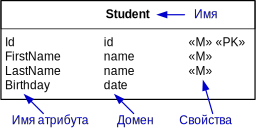
\includegraphics[width=0.8\textwidth]{../assets/kgeorgiy/modelling/ERModel_Entity.svg.png}
	\caption{Иллюстрация сущности}
\end{figure}

\subsubsection{Связь}
\paragraph{Связь} связывает несколько сущностей, имеет имя и тип. Тип связи обозначается на её
концах

% На рисунке \ref{end-types} приведены типы концов связей.

\begin{figure}[h]
	\centering

	\includegraphics[width=0.8\textwidth]{../assets/kgeorgiy/modelling/ERModel_ArrowEnds.svg.png}
	\caption{Типы концов}
	%	\label{end-types}
\end{figure}

\begin{remark}
	Тут кривой рисунок, 'Один' - должна быть просто прямая линия, без значка обязательности
\end{remark}

%На рисунке \ref{ref-types} приведены типы связей.

\begin{figure}[h]
	\centering

	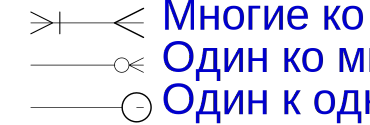
\includegraphics[width=0.8\textwidth]{../assets/kgeorgiy/modelling/ERModel_RelationshipTypes.svg.pn
		g}
	\caption{Примеры связей}
	%	\label{ref-types}
\end{figure}

\subsubsection{Ассоциации}
\paragraph{Ассоциация} это некоторое обобщение связи, два типа обобщения:
\begin{enumerate}
	\item нагрузить связть, задать ей дополнительные свойства
	\item сделать многосторонней, больше чем два конца
\end{enumerate}

\begin{figure}[h]
	\centering

	\includegraphics[width=0.8\textwidth]{../assets/kgeorgiy/modelling/ERModel_Association.svg.png}
	\caption{Пример ассоциации}
\end{figure}

\begin{remark}
	У ассоциаций, в отличии от обычных связей, есть название и атрибуты, но нет ключей, иначе они стали бы сущностями
\end{remark}

\begin{remark}
	Из-за того что у ассоциаций нет ключей, у них нет связей между собой
\end{remark}

\paragraph{Ограничения по Чену} (look-across, Chen-like), если зафиксировать все сущности кроме
одной, то получим ограничения на оставшуюся.

\paragraph{Ограничения по Мерис} (look-here Merise-like) - ограничение непосредственно на сущность

Обобщение ограничений:
\begin{figure}[h]
	\centering

	\includegraphics[width=0.8\textwidth]{../assets/kgeorgiy/modelling/ERModel_Multi_Generic.svg.png}
	\caption{Generic}
\end{figure}

\subsubsection{Слабая сущность}
Сущность, на которую можно сослаться, но у неё недостаточно атрибутов для её идентификации. Поэтому для слабой сущности вводится понятие идентифицирующей связи (которые рисуются двойной линией).
